% -----------------------------*- LaTeX -*------------------------------
\documentclass[12pt]{report}
\usepackage{%
	amsfonts,%
	amsmath,%	
	amssymb,%
	amsthm,%
	algorithm,%
	babel,%
	bbm,%
	etex,%
	%biblatex,%
	caption,%
	centernot,%
	color,%
	dsfont,%
	enumerate,%
	epsfig,%
	epstopdf,%
	geometry,%
	graphicx,%
	hyperref,%
	latexsym,%
	mathtools,%
	multicol,%
	pgf,%
	pgfplots,%
	pgfplotstable,%
	pgfpages,%
	proof,%
	psfrag,%
	subfigure,%	
	tikz,%
	ulem,%
	url%
}	
\usepackage[noend]{algpseudocode}
\usepackage[mathscr]{eucal}
\usepgflibrary{shapes}
\usetikzlibrary{%
  	arrows,%
	backgrounds,%
	chains,%
	decorations.pathmorphing,% /pgf/decoration/random steps | erste Graphik
	decorations.text,%
	matrix,%
  	positioning,% wg. " of "
  	fit,%
	patterns,%
  	petri,%
	plotmarks,%
  	scopes,%
	shadows,%
  	shapes.misc,% wg. rounded rectangle
  	shapes.arrows,%
	shapes.callouts,%
  	shapes%
}

\theoremstyle{plain}
\newtheorem{thm}{Theorem}[section]
\newtheorem{lem}[thm]{Lemma}
\newtheorem{prop}[thm]{Proposition}
\newtheorem{cor}[thm]{Corollary}

\theoremstyle{definition}
\newtheorem{defn}[thm]{Definition}
\newtheorem{conj}[thm]{Conjecture}
\newtheorem{exmp}[thm]{Example}
\newtheorem{assum}[thm]{Assumptions}
\newtheorem{axiom}[thm]{Axiom}

\theoremstyle{remark}
\newtheorem{rem}{Remark}
\newtheorem{note}{Note}
\newtheorem{fact}{Fact}

\newcommand{\norm}[1]{\left\lVert#1\right\rVert}
\newcommand{\indep}{\!\perp\!\!\!\perp}
\DeclarePairedDelimiter\abs{\lvert}{\rvert}%
\newcommand\numberthis{\addtocounter{equation}{1}\tag{\theequation}}
\newcommand{\tr}{\operatorname{tr}}
\newcommand{\R}{\mathbb{R}}
\newcommand{\N}{\mathbb{N}}
\newcommand{\E}{\mathbb{E}}
\newcommand{\Z}{\mathbb{Z}}
\newcommand{\B}{\mathscr{B}}
\newcommand{\C}{\mathcal{C}}
\newcommand{\T}{\mathscr{T}}
\newcommand{\F}{\mathcal{F}}
\newcommand{\G}{\mathcal{G}}
%\newcommand{\ba}{\begin{align*}}
%\newcommand{\ea}{\end{align*}}
\DeclareMathOperator*{\argmax}{arg\,max}
\renewcommand{\qedsymbol}{$\blacksquare$}
\makeatletter
\def\BState{\State\hskip-\ALG@thistlm}
\makeatother

\makeatletter
\def\th@plain{%
  \thm@notefont{}% same as heading font
  \itshape % body font
}
\def\th@definition{%
  \thm@notefont{}% same as heading font
  \normalfont % body font
}
\makeatother
\date{}
\usepackage{graphicx}
\graphicspath{ {Figures/} }
\usepackage{scribe_e1244}
\usepackage{times}
%\newtheorem{defn}[thm]{Definition}
%\newtheorem{lem}{Lemma}[thm]
%\newenvironment{definition}[1][Definition]{\begin{trivlist}
%\item[\hskip \labelsep {\bfseries #1}]}{\end{trivlist}}
\begin{document}

% \course{CS 497}			% optional
% \coursetitle{Geometric Data Structures} % optional
% \semester{Fall 1998}			% optional
\lecturer{Aditya Gopalan}		% optional, put lecturer's name here
\scribe{Manu Krishnan K. \& Murali K.R.}		% required, put your name here
\lecturenumber{5}			% required, must be a number
\lecturedate{January 17}		% required, omit year
\maketitle

% ----------------------------------------------------------------------



\section{Neyman-Pearson criterion for hypothesis testing}
%\subsubsection{Detection}
The Bayesian hypothesis testing assumed a prior for the hypotheses and a specific cost structure was imposed to find out the optimal decision rule. Similarly, in the minimax formulation, prior probabilities were not assumed, but the optimal rule still required a cost structure. In more general problems, which does not allow the imposition of a specific cost structure, a more elementary design criterion called the {\itshape Neyman-Pearson criterion} is adopted.\\


\begin{defn}
 A (randomized) decision rule is a map $ \delta \colon \Gamma \rightarrow [0,1]$
with the interpretation that upon seeing an observation $ $y$\in \Gamma $, output $\mathbbm{H}_1$, with probability $\delta($y$)$.\\
\end{defn}


\begin{defn}
{\itshape Type 1 error/False alarm}: Error when $\mathbbm{H}_1$ is output, but $\mathbbm{H}_0$ is the true hypothesis. The false alarm probability is denoted by $P_F(\delta)$.\\
\end{defn}



\begin{defn}
{\itshape Type 2 error/False negative/Missed detetcion}: Error when $\mathbbm{H}_0$ is output, but $\mathbbm{H}_1$ is the true hypothesis. The missed detection probability is denoted by $P_M(\delta)$. The corresponding probability of detection $P_D(\delta)=1-P_M(\delta)$\\
\end{defn}

Formally, $$P_F(\delta)=\mathbbm{P}_0(\delta\quad outputs\quad 1)=\mathbbm{E}_0[\delta(y)]$$

$$P_M(\delta)=\mathbbm{E}_1[1-\delta(y)]=1-\mathbbm{E}_1[\delta(y)]$$



\section{Neyman-Pearson problem}
For a given $\alpha \in [0,1]$, the Neyman-Pearson problem is
\begin{equation}
\smash{\displaystyle\max_\delta} P_D(\delta) \quad s.t. \quad P_F(\delta)\leq\alpha
\end{equation}
Any rule satisfying the inequality $P_F(\delta)\leq \alpha $ is called {\itshape level-$\alpha$ rule} and that which exactly achieves the equality is called {\itshape size-$\alpha$ rule}. The probability of detection is also called the {\itshape power of $\delta$}. Thus,the Neyman-Pearson problem can be restated as {\itshape "Find the most powerful level-$\alpha$ test"}.
\subsection{Basic intuition about solving eqn. 5.1}
Consider a finite observation space $\Gamma=\{y_1,y_2,..,y_n\}$. Assume that $\mathbbm{H}_0$ has a distribution $\mathbbm{P}_0$ and $\mathbbm{H}_1$, $\mathbbm{P}_1$. 

Decision rule is
$$\delta\colon\{y_1,y_2....y_n\}\rightarrow[0,1]$$
$$P_D(\delta)=\sum\limits_{i=1}^n\delta(y_i){p}_1(y_i)$$
$$P_F(\delta)=\sum\limits_{i=1}^n\delta(y_i){p}_0(y_i)$$
The problem is 
\begin{equation}
\smash{\displaystyle\max_{\delta(y_i)}} \sum\limits_{i=1}^n\delta(y_i)p_1(y_i) \quad s.t. \sum\limits_{i=1}^n\delta(y_i){p}_0(y_i)\leq\alpha
\end{equation}
which is linear program. Multiplying and dividing by $p_0(y_i)$, we have $$\smash{\displaystyle\max_{\delta(y_i)}}\sum\limits_{i=1}^n\delta(y_i)\dfrac{p_1(y_i)}{p_0(y_i)}p_0(y_i)\quad s.t.\quad  \sum\limits_{i=1}^n\delta(y_i)p_0(y_i) \leq\alpha$$
\begin{equation}
\smash{\displaystyle\max_{\delta(y_1),\delta(y_2),..,\delta(y_n)}}\sum\limits_{i=1}^n\delta(y_i) L(y_i)p_0(y_i)\quad s.t. \quad \sum\limits_{i=1}^n\delta(y_i)p_0(y_i) \leq\alpha
\end{equation}
where $\mathbbm{L}(y_i)=\dfrac{p_1(y_i)}{p_0(y_i)}$ is the likelihood ratio.
If we interpret $\alpha$ as the capacity of a knapsack, $p_0(y_i)$ as the volume of an item $y_i$ and $p_1(y_i)$ as the value of the item, then eqn.(5.3) is nothing but a knapsack problem. The solution to the problem is: Arrange the items by the decreasing order of $L(y_i)$(value per volume) and select from the highest to the lowest.
\section{Neyman-Pearson Lemma}
Consider testing $\mathbbm{H}_0$ vs $\mathbbm{H}_1$ with distributions $\mathbbm{P}_0$ and $\mathbbm{P}_1$ respectively. Let $\alpha \in [0,1]$ be a given level.
\vskip .25cm
1)(OPTIMALITY) Let $\delta$ be any decision rule of the following form:
\begin{equation}
\delta(y)=\begin{cases}
    1, & \text{if  $L(y)>\eta$}\\
    \gamma(y), & \text{if $L(y)=\eta$}\\
    0, & \text{if $L(y)<\eta$}
  \end{cases}
\end{equation}
where $\eta\geq0$ and $0\leq\gamma\leq1$ are such that $P_F(\delta)=\alpha$  ,then $\delta$ solves the Neyman-Pearson problem eqn.(5.1).
\vskip .25cm
2)(EXISTENCE) For any $\alpha\in[0,1]$,$\exists$ a rule $\delta_{NP}$ of the form eqn.(5.4) with $P_F(\delta_{NP})=\alpha$ and $\gamma(y)=\gamma_0\in[0,1]$.
\vskip .25cm
3)(UNIQUENESS) Suppose $\delta^\prime$ is any level-$\alpha$ NP rule (i.e. it solves eqn.(5.1)), then $\delta^\prime$ must be of the form eqn.(5.4), except possibly on a subset of outcomes $\tilde{\Gamma}\subseteq\Gamma$ which has $\mathbbm{P}_0(\tilde{\Gamma})=\mathbbm{P}_1(\tilde{\Gamma})=0$.
\begin{proof}
1)(OPTIMALITY) Let $\delta$ be a rule as assumed in eqn.(5.4). Let $\tilde{\delta}$ be any rule satisfying the constraint $P_F(\tilde{\delta})\leq\alpha$. We need to show that:$$P_D(\delta)\geq P_D(\tilde{\delta})$$
Observe that, $\forall y\in\Gamma$ \\

$[\tilde{\delta}(y)-\delta(y)][p_1(y)-\eta p_0(y)]\leq0$\\

$\Longrightarrow\int\limits_\Gamma(\tilde{\delta}(y)-\delta(y))(p_1(y)-\eta p_0(y))dy\leq0$\\

$\Longleftrightarrow\int\limits_\Gamma\tilde{\delta}(y)p_1(y)dy-\int\limits_\Gamma{\delta(y)}p_1(y)dy-\eta(\int\limits_\Gamma\tilde{\delta}(y)p_0(y)dy-\int\limits_\Gamma{\delta(y)}p_0(y)dy)\leq0$\\

$\Longleftrightarrow P_D(\tilde{\delta})-P_D(\delta)-\eta(P_F(\tilde{\delta})-P_F(\delta))\leq0$\\

$\Longleftrightarrow P_D(\tilde{\delta})-P_D(\delta) \leq \eta(P_F(\tilde{\delta})-P_F(\delta))$\\

$\leq0$ (by assumption)\\

$\Longrightarrow P_D(\delta)\geq P_D(\tilde{\delta})$\\

2)(EXISTENCE) We will exhibit $\gamma_0\in[0,1]$ and $\eta_0\geq 0$, s.t. the rule 
\begin{equation}
\delta(y)=\begin{cases}
    1, & \text{if  $L(y)>\eta_0$}\\
    \gamma_0, & \text{if $L(y)=\eta_0$}\\
    0, & \text{if $L(y)<\eta_0$}
  \end{cases}
\end{equation}
This rule achieves $P_F(\delta)=\alpha$\\
Let $\eta_0\coloneqq\smash{\displaystyle\min_{\eta}}\{\eta\geq 0\colon \mathbbm{P}_0(L(y)>\eta)\leq\alpha)$
\begin{figure}[H]
 \centering
 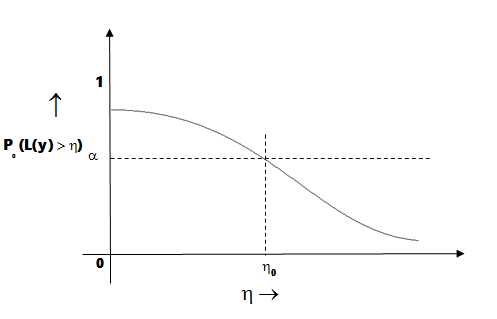
\includegraphics{Case1}
 \caption{Case 1}
\end{figure}
\begin{figure}[H]
 \centering
 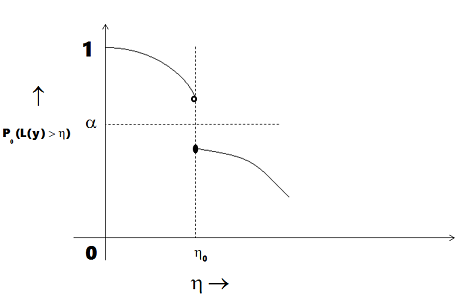
\includegraphics{Case2}
 \caption{Case 2}
\end{figure}
{\bfseries Case 1:}(when the ccdf is nice) Select $\gamma_0$ arbitrarily.\\
\vskip .2cm
{\bfseries Case 2:}(when there is a jump discontinuity in ccdf) Select $\gamma_0=\dfrac{\alpha-\mathbb{P}_0(\mathbb{L}(y)>\eta_0)}{\mathbb{P}_0(\mathbb{L}(y)=\eta_0)}$\\
Thus,\\
 $P_F(\delta_{NP})=\mathbb{E}_0(\delta_{NP})=1\mathbb{P}_0(\mathbb{L}(y)>\eta_0)+\gamma_0\mathbb{P}_0(\mathbb{L}(y)=\eta_0)$\\
\vskip .2cm
$\Longrightarrow P_F(\delta_{NP})=\alpha$, in both the cases.\\

3)(UNIQUENESS) With $\alpha\in[0,1]$, suppose $\delta^\prime$ solves the NP problem(eqn.(5.1)), let $\delta$ be a rule of the form (eqn.(5.4)) with $P_F(\delta)=\alpha$ (by EXISTENCE), we have $P_D(\delta)=P_D(\delta^\prime)$ (by assumption). Also, \\
\vskip .2cm
$P_D(\delta^\prime)-P_D(\delta)\leq\eta(P_F(\delta^\prime)-P_F(\delta))$\\
\vskip .2cm
$\Longrightarrow 0\leq\eta(P_F(\delta^\prime)-P_F(\delta))\leq 0$\\
\vskip .2cm
$\Longrightarrow P_F(\delta^\prime)=\alpha $\\
\vskip .2cm
$\int\limits_\Gamma[\delta^\prime(y)-\delta(y)][p_1(y)-\eta p_0(y)]dy=0$\\
As seen previously, the integrand is non-negative and hence it is zero except possibly on outcomes of zero probability under the hypotheses. Thus $\delta^\prime$ has the form of the template rule $\delta$ except possibly in the $\{y\in\Gamma\colon\mathbb{L}(y)=\eta\}$.
\end{proof}

\end{document}

